\documentclass[
	12pt,				% tamanho da fonte
	openright,			% capítulos começam em pág ímpar (insere página vazia caso preciso)
	oneside,			% para impressão apenas em um lado do papel
	a4paper,			% tamanho do papel.
	brazil				% o último idioma é o principal do documento
	]{abntex2}

\usepackage{etoolbox}
\usepackage{lmodern}			% Usa a fonte Latin Modern			
\usepackage[T1]{fontenc}		% Selecao de codigos de fonte.
\usepackage[utf8]{inputenc}		% Codificacao do documento (conversão automática dos acentos)
%\usepackage{lastpage}			% Usado pela Ficha catalográfica
\usepackage{indentfirst}		% Indenta o primeiro parágrafo de cada seção.
\setlength{\parindent}{1.5cm}   % Espaçamento de 1,5cm do parágrafo
\usepackage{color}				% Controle das cores
\usepackage{graphicx}			% Inclusão de gráficos
\usepackage{microtype} 			% para melhorias de justificação
\usepackage{lipsum}				% para geração de dummy text
\usepackage{abntex2cite}	% Citações padrão ABNT
\usepackage[table,xcdraw]{xcolor}% Cédula colorida em tabelas
%\usepackage{pdflscape}          % Rotaciona página
\usepackage{Capa}               % Capa e folha de rosto com modificações
\usepackage{float}              % Melhor posicionamento de figuras
\usepackage{gensymb}            % símbolo º
\usepackage[justification=justified,singlelinecheck=false]{caption}
%\usepackage{etoolbox}           % Configurações adicionais de macros
\usepackage{xparse}						
\usepackage{multirow}
\NewDocumentCommand\cc{+u{\cc}}{\ignorespaces}
\usepackage[justification=centering]{caption}
\usepackage{listings}

% --------------------
% Dados do Documento
% --------------------

\lstset{
  basicstyle=\ttfamily,
  keywordstyle=\color{blue},
  commentstyle=\color{green},
  stringstyle=\color{red},
  numbers=left,
  numberstyle=\tiny\color{gray},
  stepnumber=1,
  numbersep=5pt,
  showspaces=false,
  showstringspaces=false,
  tabsize=2,
  breaklines=true,
  breakatwhitespace=false
}
\titulo{Projeto de um circuito integrado de um pré-distorcedor digital baseado em polinômio de
memória}
\autor{Leonardo de Andrade Santos}
\data{\the\year}
\instituicao{Universidade Federal do Paraná}
\local{Curitiba}
\orientador[Orientadora:]{Sibilla Batista da Luz França}
\coorientador[Coorientador:]{Eduardo Gonçalves de Lima}
\preambulo{Trabalho de conclusão de curso do Curso de Graduação em Engenharia Elétrica da Universidade Federal do Paraná, como exigência parcial para obtenção do grau de Bacharel em Engenharia Elétrica.}


% ---------------------
% Configurações básicas
% --------------------

% informações do PDF
\makeatletter

\hypersetup{
     	%pagebackref=true,
		pdftitle={\@title},
		pdfauthor={\@author},
    	pdfsubject={\imprimirpreambulo},
        pdfkeywords = {Desempenho Acadêmico}{Estatística Descritiva}{Evasão}{Vestibular},
		colorlinks=true,       		% false: boxed links; true: colored links
    	linkcolor=black,          	% color of internal links
    	citecolor=black,      	    % color of links to bibliography
    	filecolor=magenta,      	% color of file links
		urlcolor=black,
		bookmarksdepth=4
}
\makeatother

\graphicspath{{Figuras/}}

% -------------------
% Início do documento
% -------------------

\begin{document}

\frenchspacing % Retira espaço extra obsoleto entre as frases.

% ----------------------------------------------------------
% ELEMENTOS PRÉ-TEXTUAIS
% ----------------------------------------------------------

% ----
% Capa
% ----
\imprimircapa
% ---

% --------------
% Folha de rosto
% --------------
\imprimirfolhaderosto
% ---

%\begin{dedicatoria}  % Opcional
%\vspace*{\fill}
% Dedico este trabalho aos meus pais .....
%\vspace*{\fill}
%\end{dedicatoria}

% --------------
% Agradecimentos  % Opcional
% --------------

% \begin{agradecimentos}

% Inclua seus agradecimentos aqui. Há vários exemplos na internet.
% \end{agradecimentos}

% \begin{epigrafe} % Opcional
% \vspace*{\fill}
% \begin{flushright}
% \textit{"Democracia é oportunizar a todos o mesmo ponto de partida. \\
%          Quanto ao ponto de chegada, depende de cada um".\\
%          (Fernando Sabino)}
% \end{flushright}
% \end{epigrafe}

% ------
% Resumo
% ------
\newpage
\setlength{\absparsep}{18pt}   % ajusta o espaçamento dos parágrafos do resumo
\setlength{\abstitleskip}{1cm} % adiciona mais um cm após o 'titulo' do Resumo para ficar com 2cm,

\begin{resumo}

A evolução dos sistemas de comunicação sem fio acarretou na implementação de diversas aplicações móveis e sem fio como desenvolvimento web, aplicação IoT, entre outros. Neste cenário, melhorar a eficiência energética se torna uma alternativa desejável tanto para os dispositivos móveis que buscam melhorar a autonomia das suas baterias, quanto para as estações de rádio base, que buscam reduzir sues desperdício em perdas de calor. No entanto, uma melhor eficiência energética implica em uma menor linearidade nos sistemas de amplificação de sinais, presentes nos sistemas transmissores de sinais de rádio. Isto é importante de ser ressaltado, pois a banda reservada para aplicações móveis é reduzida, de forma que para se alcançar maiores taxas de transmissão é necessário alternar estratégias de modulação tanto da fase, quanto da amplitude da onda portadora. E essas duas condições são conflitosas, já que a modulação AM é sensível a linearidade de forma que quanto mais linear um sistema ocorrem menos erros de transmissão. Sendo assim, uma alternativa para contornar esse obstáculo, que é implementar um sistema, eficiente energeticamente e linear é a implementação de um DPD em cascata com um PA. Portanto, o objetivo deste trabalho de conclusão de curso é o design de um circuito integrado dedicado de um DPD. Para atingir esse objetivo esse projeto foi divido em quatro etapas, o estudo e modelagem dos DPDs, modelagem do DPD em software, implementação do DPD em FPGA e finalmente o design do circuito integrado do DPD. Para a modelagem do DPD foi utilizada a métrica do NMSE, nela quanto menor o NMSE encontrado mais fiel e o modelo com a realidade. Sendo assim, na etapa de modelagem do PA alcançou-se um NMSE de -23.57 db. Em seguida, foi feita o levantamento do número de bits necessários para a realização desses cálculos de forma a minimizar o NMSE, para isso foi verificado que com apenas 8 bits de resolução do sinal já foi possível alcançar um NMSE próximo do valor alcançado em virgula flutuante. Portanto, ainda restam as etapas de implementação do DPD em FPGA e o design do circuito integrado. 

\textbf{Palavras-chave}: VHDL, FPGA, DPD 

.
\end{resumo}

% -------------------------------
% Lista de abreviaturas e siglas - Opcional
% -------------------------------

\begin{siglas}  %
 \item[DPD]  Pré-Distorcedor Digital
 \item[FPGA] Matriz de Portas Programáveis em Campo 
 \item[PA] Amplificador de Potência
 \item[RF] Rádio Frequência 
 \item[PARF] Amplificador de Potência de Rádio Frequência 
 \item[HDL] Linguagem de Descrição de software
 \item[VHSIC]  Circuito integrado de Velocidade Muito Elevada 
 \item[VHDL]  VHSIC Hardware Description Language
\end{siglas}

\listoffigures*
\cleardoublepage
% -------
% Sumario
% -------
\pdfbookmark[0]{\contentsname}{toc}
\tableofcontents*
\cleardoublepage
% ---

\makepagestyle{abntheadings}
\makeevenhead{abntheadings}{\ABNTEXfontereduzida\thepage}{}{}
\makeoddhead{abntheadings}{}{}{\ABNTEXfontereduzida\thepage}
\makeheadrule{abntheadings}{\textwidth}{0in}

% ----------------------------------------------------------
% ELEMENTOS TEXTUAIS
% ----------------------------------------------------------

\textual

\setcounter{page}{1}

\chapter{Introdução}
A evolução dos sistemas de comunicação móveis, impulsionada pela crescente demanda por comunicações mais rápidas e eficientes, tem levado à implementação de uma variedade de serviços, incluindo aplicações multimídia, desenvolvimento web e aplicações IoT \cite{John2016}. No entanto, essa evolução também trouxe desafios significativos, como a necessidade de melhorar a eficiência energética, tanto para dispositivos móveis, visando aumentar a autonomia da bateria, quanto para estações de rádio base, visando reduzir o consumo de energia devido às perdas de calor. Para atender a essas demandas, estratégias de modulação que alteram tanto a fase quanto a amplitude de ondas portadoras em radiofrequência se tornaram essenciais \cite{Kenington2000}. Além disso, a modulação na amplitude requer linearidade na transmissão para evitar erros e interferências na comunicação entre usuários vizinhos \cite{Cripps2006}. Essa complexa tarefa recai sobre o projetista do PARF, que enfrenta o desafio de desenvolver um hardware eficiente em termos energéticos e linear ao mesmo tempo, uma vez que esses dois objetivos podem entrar em conflito \cite{Chavez2018}. Uma solução para contornar esse desafio é a implementação de um pré-distorcedor de Sinais Digital em Banda Base, que visa compensar a distorção causada pelo PARF \cite{Cripps2006}. O DPD é conectado em cascata ao PARF e requer um modelo de alta precisão e baixa complexidade computacional para representar as características de transferência direta e inversa do PARF. Existem duas abordagens para modelar o PARF: modelos físicos, que são detalhadas e computacionalmente complexos, e modelos empíricos, que se baseiam em medições de entrada e saída do PARF, com menor complexidade computacional, mas com uma possível diminuição da precisão. Devido às exigências rigorosas de frequência de operação, a paralelização das operações torna-se essencial, e os Arranjos de Portas Programáveis em Campo emergem como uma alternativa viável para a implementação de circuitos pré-distorcedores \cite{Pedroni2010}. As FPGAs são dispositivos lógicos programáveis que permitem a reconfiguração física de componentes de eletrônica digital, acelerando processos e suportando operações paralelas e sequenciais. Neste contexto esse projeto foi planejado com os seguintes objetivos geral e específicos

\section{Objetivo Geral}
O desenvolvimento de um circuito integrado dedicado para um pré-distorcedor digital na tecnologia BiCMOS 130 nm 8HP.
\section{Objetivos Específicos}

Para alcançar o objetivo geral, este trabalho foi desenvolvido com base nos seguintes objetivos específicos:

\begin{enumerate}
    \item Modelar com precisão o PA em software;
    \item Modelar o DPD em software a partir da modelagem do PA;
    \item Implementar o DPD em hardware utilizando uma HDL;
    \item Desenvolver o design do circuito integrado.
\end{enumerate}



\chapter{Revisão de Literatura}
O sistema de comunicação pode ser divido em 3 sub-sistemas principais:
\begin{itemize}
    \item Meio transmissor;
    \item Receptor;
    \item Transmissor;
\end{itemize}
No entanto, este trabalho foca exclusivamente no sistema transmissor, ilustrado pela figura \ref{fig:sistemadetrasmissao}, onde observa-se diversos elementos de que compõem o transmissor de sinal e dentre esses elementos tem-se que o amplificador de sinal é o componente de maior demanda energética, por se tratar do componente que converte a energia da fonte em energia irradiada pela antes de transmissão. Então para que o sistema de transmissão atue de maneira eficiênte é imprescindível que o trasmissor atue da maneira mais eficiênte o possivel. 

% // TODO Refazer figura
\begin{figure}[h!]
    \centering
    \captionsetup{justification=centering}
    \caption*{Fonte: autor}
    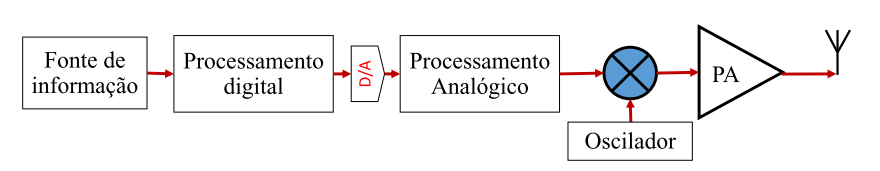
\includegraphics[width=0.5\textwidth]{sistematrasmissorpng.png}
    \caption{Sistema de transmissão simplificado}
    \label{fig:sistemadetrasmissao}
\end{figure}


\chapter{Material e Métodos}
Conforme dito anteriormente o trabalho busca o desenvolvimento do design do circuito integrado de um DPD, a partir de um modelo validado em software, e em hardware, no caso, FPGA. Para isso esse projeto foi divido em 4 etapas principais:

\begin{itemize}
    \item Estudo DPD;
    \item Implementação em software;
    \item Implementação em FPGA;
    \item Design e validação do circuito integrado.
\end{itemize}

O cronograma para o desenvolvimento dessas atividades esta disponivel na tabela \ref{tab:cronograma} a seguir:

\begin{table}[ht!]
    \centering
    \renewcommand{\arraystretch}{0.8} % Diminui a altura das linhas
    \setlength{\tabcolsep}{4pt} % Diminui o espaçamento horizontal das células
    \begin{tabular}{|l|c|c|c|c|c|c|c|c|c|}
    \hline
    & mar/24 & abr/24 & mai/24 & jun/24 & jul/24 & ago/24 & set/24 & out/24 & nov/24\\
    \hline
    Etapa 1 & \cellcolor{yellow} & \cellcolor{yellow} &&&&&&& \\
    \rowcolor{gray!20} % Cor da linha
    Etapa 2 && \cellcolor{yellow} & \cellcolor{yellow} & \cellcolor{yellow} &&&&&\\
    Etapa 3 &&& \cellcolor{yellow} & \cellcolor{yellow} & \cellcolor{yellow} & \cellcolor{yellow} &&&\\ 
    \rowcolor{gray!20} % Cor da linha
    Etapa 4 &&&&&& \cellcolor{yellow}& \cellcolor{yellow} & \cellcolor{yellow} & \cellcolor{yellow}\\ 
    \hline
\end{tabular}
\caption{Cronograma de Etapas}
\label{tab:cronograma}
\end{table}
    

\section{Estudo dos DPDs}
A etapa consistiu no estudo dos DPDs, conforme apresentado no Capítulo \ref{chap:revi}, onde foi feito todo o levantamento sobre os tipos de modelagem dos DPDs. O objetivo deste estudo é entender as diferentes abordagens de modelagem, avaliar seus desempenhos e identificar as mais adequadas para a aplicação em amplificadores de potência.

\section{Implementação em software}

Nesta etapa, foi realizada a implementação do modelo DPD em software, utilizando a linguagem de programação Python. Python é uma linguagem amigável, amplamente difundida na comunidade acadêmica e prática de usar.

Para essa modelagem, foram coletados sinais de entrada e saída de um amplificador de potência classe AB, que utiliza um HEMT fabricado com tecnologia GaN. O amplificador foi excitado por um sinal portador de frequência de 900 MHz, modulado por um sinal de envelope WCDMA 3GPP com aproximadamente 3,84 MHz de largura de banda. Os dados de entrada e saída do amplificador de potência foram medidos usando um VSA Rohde \& Schwarz FSQ com uma taxa de amostragem de 61,44 MHz, conforme disponível em \cite{Bonfim2016}.

A seguir, foi realizado o cálculo da estimativa do sinal utilizando números com vírgula fixa. Para verificar a precisão dessa estimativa em relação ao sinal original, foi calculado o NMSE. Para essa validação, os dados foram inicialmente divididos em conjuntos de extração e validação. A matriz de confusão foi calculada com os dados de extração, conforme descrito na seção \ref{sub:polimem}, utilizando o código disponível no anexo \ref{cod:mp}. Esse cálculo é essencial para a extração dos coeficientes do polinômio de memória. Após a extração dos coeficientes, foi calculado o modelo do PA, que foi então validado com os dados de validação. O NMSE obtido para um polinômio de 2° grau com uma amostra memorizada foi de -23,57 dB.

Em seguida, o algoritmo foi ajustado para operar com números em vírgula fixa e o número total de bits foi reajustado para atingir a menor resolução possível, buscando o menor NMSE simulado, conforme ilustrado pelo anexo \ref{cod:mpint}, perceba que por ser tratar de um calculo em virgula flutuante, foi necessário fazer uma readequação do resultado obtido entre cada multiplicação de forma a manter a resolução inicial.

\section{Implementação em FPGA}
Essa etapa conssise no desenvolvimento do DPD do polinomio de memória 

\section{Design e validação}
Finalmente, na última etapa, realiza-se o processo de concepção do circuito integrado do DPD como um circuito dedicado integrado na tecnologia BiCMOS 130 nm 8HP, utilizando as ferramentas do Cadence.
O fluxo de projeto VLSI  para design de um circuito integrado de aplicação específica, inclui a descrição do circuito em VHDL, síntese lógica utilizando as células padrão da tecnologia, place and route e simulações comportamentais e temporais. O diagrama do fluxo VLSI pode ser ilustrado pela figura \ref{fig:CMOS2010}.

\begin{figure}[ht!]
    \centering
    \captionsetup{justification=centering}
    \caption*{Fonte: \cite{CMOS2010}}
    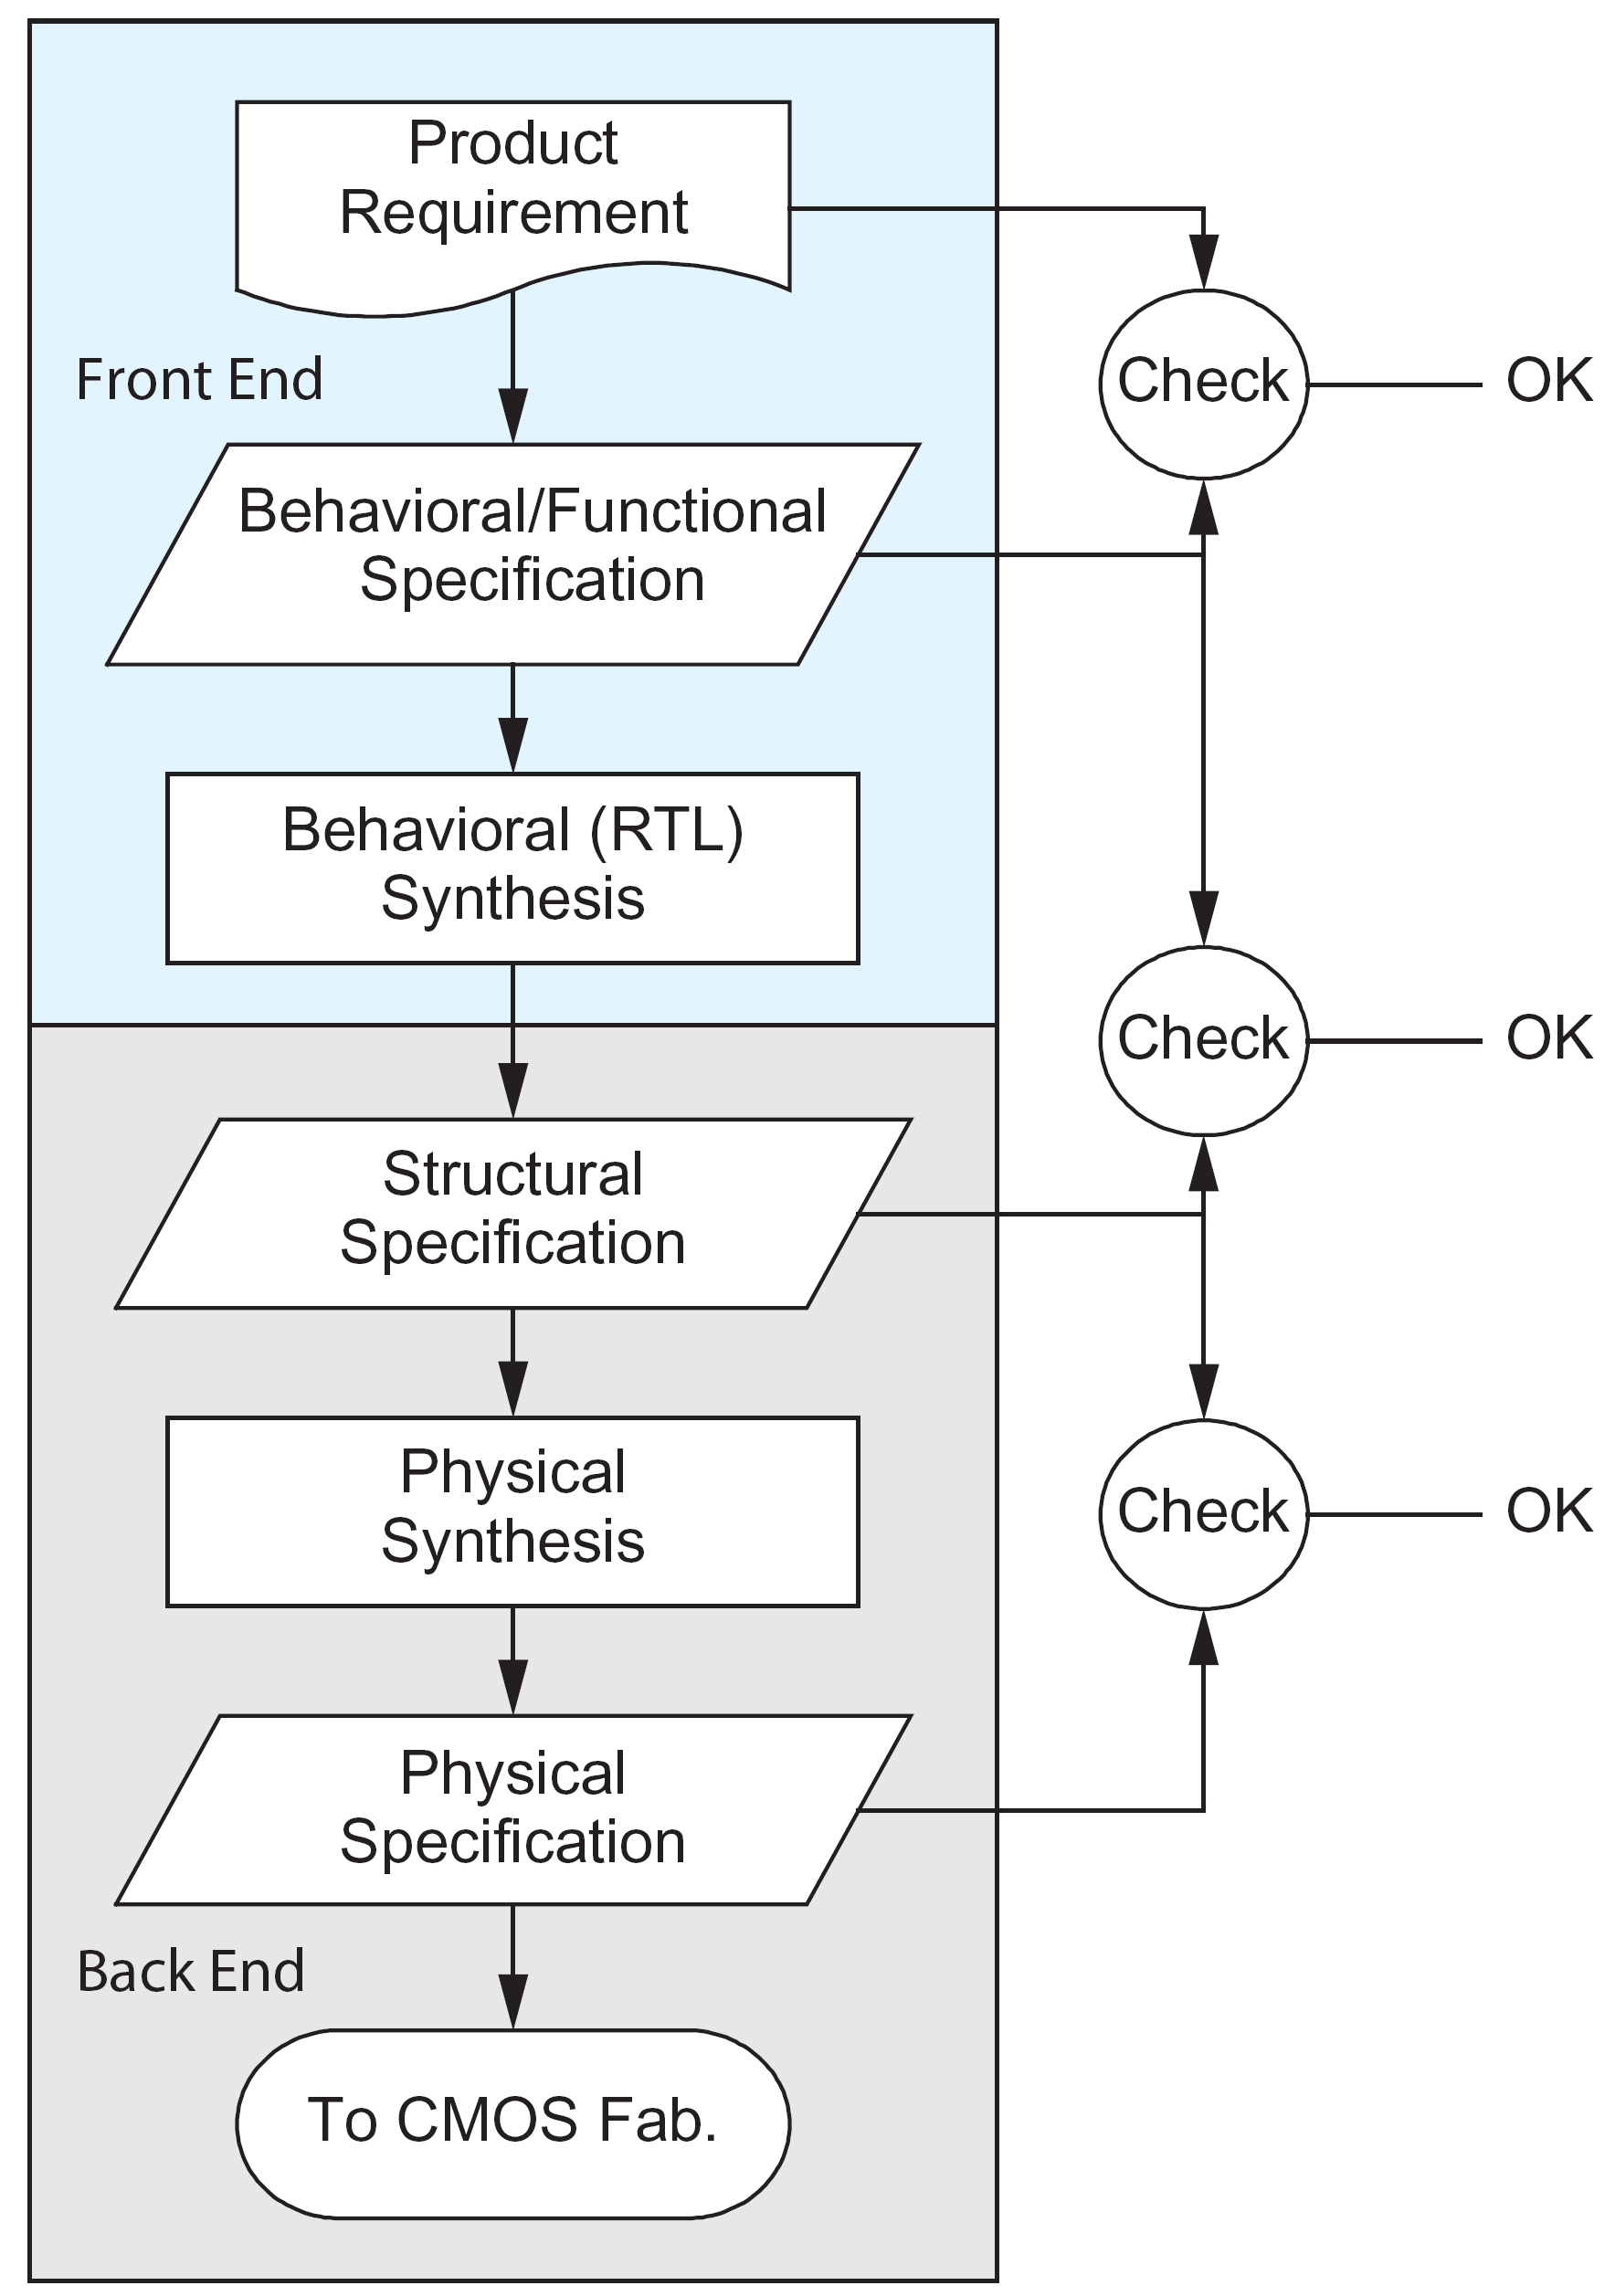
\includegraphics[width=0.5\textwidth]{fluxovlsi.png}
    \caption{Fluxo de projeto VLSI}
    \label{fig:CMOS2010}
\end{figure}

No processo de desenvolvimento do circuito, várias etapas são executadas. Primeiro, há a simulação comportamental para verificar se o circuito VHDL atende às expectativas, utilizando um testbench em VHDL e a ferramenta Cadence NCLaunch. Em seguida, ocorre a síntese lógica, onde a partir do modelo comportamental, utiliza-se a ferramenta Genus para criar um modelo RTL com células padrão de tecnologia específica, considerando restrições de área, frequência e consumo de energia. A síntese gera dois arquivos: um com componentes e conexões, em Verilog, e outro com informações de atraso no formato SDF. A simulação pós-síntese é realizada para validar o netlist gerado, usando o mesmo testbench da simulação comportamental. Em seguida, na etapa de PAR, o layout é criado posicionando as células e realizando as conexões entre essas células, utilizando a ferramenta Innovus. Por fim, na simulação pós-PAR, o circuito é simulado considerando as resistências e capacitâncias parasitas. Cada etapa é fundamental para garantir o correto funcionamento do circuito.



\chapter{Resultados e Discussão}
Conforme dito no capitulo \ref{chap:mati} o trabalho foi divido em 4 etapas, nas quais a primeira etapa consistiu no estudo dos DPDs e nos métodos de modelagem deles, a segunda etapa consistiu na implementação desta modelagem em software, que foi optado em utilizar o python, a etapa 3 que consiste na implementação do modelo de DPD escolhido em hardware ultilizando a linguagem VHDL e finalmente na quarta etapa e feita o design do circuito integrado do circuito integrado.
Neste capitulo serão exibidos os resultados das etapas 2 ja que a etapa 1 cosiste no pesquisa bibliográfica e as etapas 3 e 4 serão desenvolvidas na segunda etapa do projeto.

\section{Etapa 2}
A etapa 2 consiste na modelagem do PA em software para posteriormente ser feito a modelagem do DPD, e finalmente ser feito o levantamento da quantidade de bits necessarios para a implementação do DPD em hardware minimizando os erros de quantização. 
O resultado desse levantamento esta presente no grafico na figura \ref{fig:bits}.
\begin{figure}[ht!]
    \centering
    \captionsetup{justification=centering}
    \caption*{Fonte: Autor}
    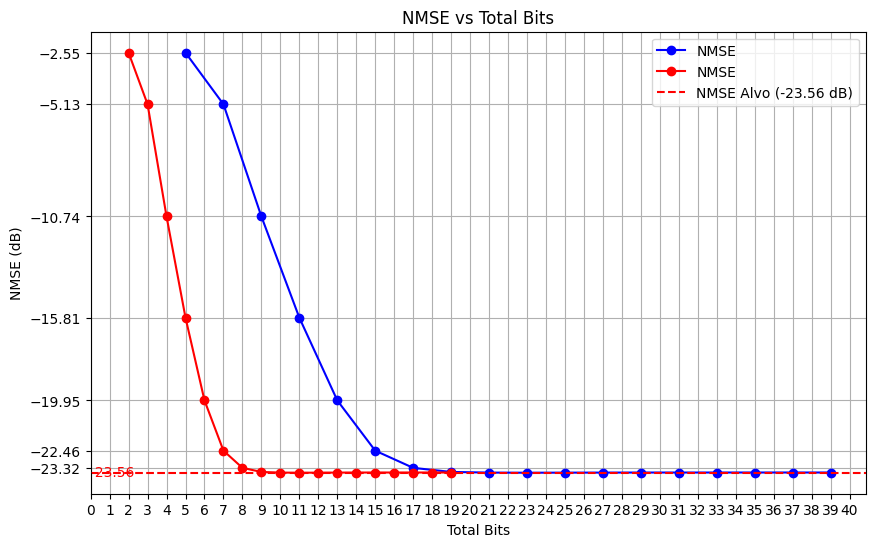
\includegraphics[width=0.5\textwidth]{bits.png}
    \caption{Grafico Numero de bits x NMSE}
    \label{fig:bits}
\end{figure}

Neste grafico observa-se que nao existe ganhos significativos no erro a partir de 7 bits, por tanto foi feito a modelagem do PA para esses 8 bits, o resultado alcançado está ilustrado pela figura \ref{fig:modelopa} a seguir.
\begin{figure}[ht!]
    \centering
    \captionsetup{justification=centering}
    \caption*{Fonte: Autor}
    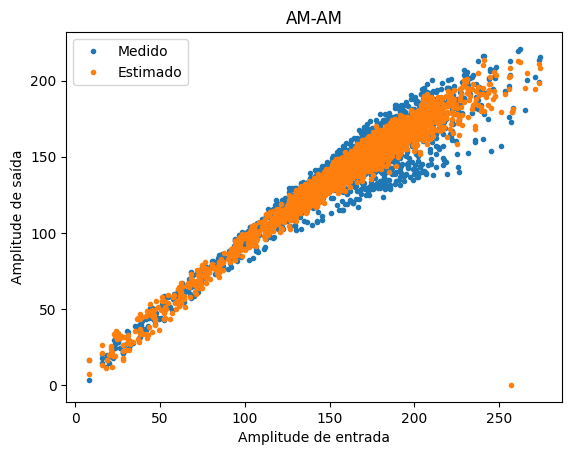
\includegraphics[width=0.75\textwidth]{modeloPA.png}
    \caption{Modelo do PA em virgula fixa}
    \label{fig:modelopa}
\end{figure}

Observando a figura \ref{fig:modelopa} observa-se que o modelo apresentou o resultado esperado e partir disso foi feito a modelagem do DPD, cujo o resultado esta ilustrado pela figura \ref{fig:modelodpd} a seguir

\begin{figure}[ht!]
    \centering
    \captionsetup{justification=centering}
    \caption*{Fonte: Autor}
    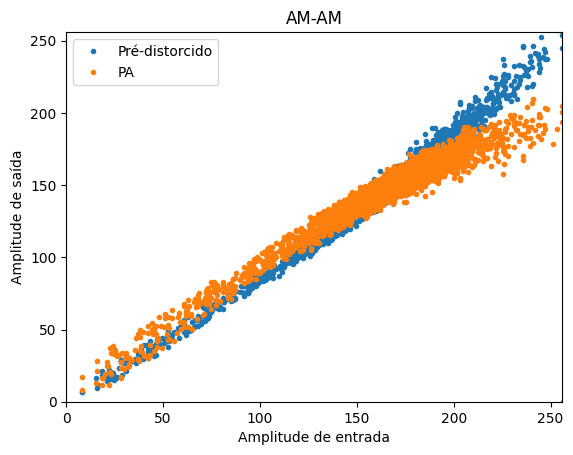
\includegraphics[width=0.75\textwidth]{modelodpd.png}
    \caption{Modelo do DPD em virgula fixa}
    \label{fig:modelodpd}
\end{figure}

\chapter{Conclusão}
Apresente as considerações finais (ou conclusões) do trabalho.

% ----------------------------------------------------------
% Referências bibliográficas
% ----------------------------------------------------------

%\setlength{\afterchapskip}{\baselineskip}

\bibliography{Referencias}

% ----------------------------------------------------------
% ELEMENTOS PÓS-TEXTUAIS
% ----------------------------------------------------------
\postextual
% ----------------------------------------------------------

% ----------------------------------------------------------
% ANEXOS
% ----------------------------------------------------------

\begin{apendicesenv}

\partapendices

\chapter*{\normalsize APÊNDICE A - Digite o cabeçalho do apêndice}

Apêndice: texto ou documento elaborado pelo autor, a fim de complementar sua argumentação, sem prejuízo da unidade nuclear do trabalho.

\chapter*{\normalsize APÊNDICE B - Digite o cabeçalho do apêndice}

\end{apendicesenv}

\begin{anexosenv}

\partanexos
%\addcontentsline{toc}{chapter}{\hspace{2.105cm}ANEXOS}
\renewcommand{\ABNTEXchapterfontsize}{\ABNTEXsectionfont}

\chapter*{\normalsize ANEXO A - Digite o cabeçalho do anexo}
\begin{lstlisting}[language = Python, caption={Código}, label={lst:hello_world}]
def hello_world():
    print("Hello, World!")
\end{lstlisting}
Anexo: texto ou documento não elaborado pelo autor, que serve de fundamentação, comprovação e ilustração.

\chapter*{\normalsize ANEXO B - Digite o cabeçalho do anexo}

\end{anexosenv}


\end{document}